\chapter{Implementace rozpoznávání gest}
Následné algoritmy byly testovány na kameře Kinect v2 s využitím nástroje  projectGenerator od openFrameworks. Program má i vývojové prostředí, ze kterého lze spoustit aplikaci. V přiloženém souboru bakalářské práce README.txt je uveden postup pro spuštění programu pomocí generátoru v příkazové řádce.

\section{Software}

OpenFrameworks~\cite{1} je open source C++ nástroj pro kreativní programování.\\
Využívá doplněk ofxKinectV2~\cite{2}. Oproti zabudovanému ofxKinect je optimalizovaný pro aktuální openFrameworks (verze 0.9.0), je stabilnější, rychlejší a podporuje pro případné potřeby i více kamer.

Kód v openFrameworks se dělí do třech hlavních částí. Jedná se o funkce \textit{setup}(), \textit{update}() a \textit{draw}(). Sekce \textit{setup} slouží pro počáteční nastavení programu, proměnných apod., \textit{update} obsahuje výpočetní a aktualizační část a \textit{draw} má na starosti vykreslování.

Program se snaží vykonávat všechny části tak často, jak to lze. V \textit{update} i \textit{draw} se může využít funkce \textit{ofGetElapsedTimef}(), která vrací vteřiny v desetinné přesnosti od spuštění programu nebo \textit{ofGetElapsedTimeMilis}(), která vrací čas od resetování čítače. Jelikož lze předpokládat, že člověk nemění gesta rychleji, než je počítač zpracovává, tak můžeme využít funkci \textit{modulo} (i jiných) a ovlivnit jak často se budou vykonávat \textit{update} a \textit{draw} nebo jejich podčásti. Funkce \textit{isFrameNew}(), která vrací binární hodnotu určující, jestli se snímek změnil či nikoliv, omezuje počet snímků, které jsou následně zpracovány, aby se neprováděly výpočty opakovaně.

% %\subsection{Měření času v OF}
%timeStart = ofGetElapsedTimef();
%	/*kód*/
%timeEnd = ofGetElapsedTimef();
% %diffTime = timeEnd - timeStart;

\section{Hardware}

K implementaci této práce byla využita kamera Kinect v2. Zdroje, ze kterých lze data využít k potřebám aplikace jsou RGB kamera s rozlišením 1920 x 1080 pixelů a kamera na snímání hloubky s rozlišením 512 x 424 pixelů.

Jedná se o relativně levnou a dostupnou kameru, jejíž cena se v době zpracování této práce (začátek roku 2018) pohybovala do tří tisíc korun.

\subsection{Výstupy z kamery}

Obě kamery poskytují užitečné informace pro účely projektu. RGB kamera nabízí pole pixelů, kde každý má složky RGB s hodnotami v intervalu 0 až 255. Lze využít v kombinaci s robustním programem, který by na základě barvy, tvarů a dalších vylučovacích prvků správně detekoval nejdříve ruku a poté i gesta. % Jedná se však o znatelně náročnější způsob.

Hloubková kamera poskytuje pole s hodnotami 0 až 255 na základě vzdálenosti objektu od kamery. Stupnice hodnot je klesající, to jest nejbližší objekty mají hodnotu 255. Ve vzdálenosti 3\,metry hodnoty klesnou na 150. 

\begin{figure}[htp]
\centering
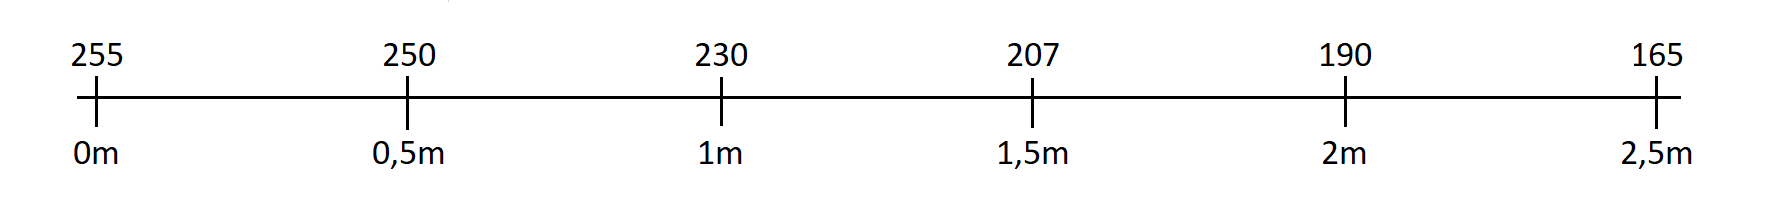
\includegraphics[width=\textwidth]{scale.png}
\caption{Stupnice hodnot, kterých nabývá hloubková kamera v závislosti na vzdálenosti}
\label{fig:scale}
\label{pic9}
\end{figure}

Minimální vzdálenost pro správné měření vzdálenosti je 0.5\,m a maximální 4.5\,m. Při větší vzdálenosti bude Kinect stále ještě detekovat objekty v zorném poli, ale bude poskytovat nepřesná data. Velký vliv má i hloubkové rozlišení, které je pro velké vzdálenosti nedostačující. V dálce 5\,m od kamery je rozlišení 7\,cm.\\

Měřené vlastnosti prostředí, které lze využít jsou vzdálenost od kamery, vzdálenost mezi jednotlivými pixely, úhly a barvy pixelů. V této bakalářské práci je kladen důraz na vzdálenosti.

\subsubsection{RGB video}
Výstupem z RGB kamery je dvoudimenzonální pole se třemi hodnotami jednotlivých barevných složek. Zpracování obrazu z RGB videa nebude v této práci využito. \\

\subsubsection{Hloubkové video}
Zpracování hodnot z hloubkové kamery je jednodušší, protože se jedná o jednodimenzionální pole s hodnotou, která reprezentuje vzdálenost. Prahování (tresholding) se pak provádí jednoduchým porovnáním hodnot a vytvoření binárního obrazu je rychlejší, než komplikované rozhodovací funkce u barevného obrazu.

Nedostatky vyplývající z využití pouze hloubkové kamery spočívají především v tom, že pokud je v záběru objekt, který má podobnou stavbu a strukturu jako je ruka, tak je mylně detekován a zpracováván.\\

\section{Postup}
Doporučený postup zpracování by měl sestávat ze čtyř částí:

\begin{enumerate}
\item úvodní nastavení,
\item nalezení ruky,
\item identifikace gesta a
\item vykreslení ruky (volitelně).
\end{enumerate}

\subsubsection{Úvodní nastavení}
Uživateli aplikace je potřeba dát na vědomí podmínky interakce. V praktické části bakalářské práce je nutné, aby byla ruka nejbližší objekt v zorném poli kamery. Alternativou může být počáteční umístění ruky doprostřed kamery, aby mohla dále vycházet z umístění za využívání historie nebo aby se zkrátila doba hledání ruky.

\subsubsection{Nalezení ruky}
V této části je prostor pro určení podmínek a způsobu vyhledávání ruky. Je vhodné nejdříve vyplnit díry vzniklé šumem v obraze a zahrnout další chyby hardwaru a vlivy okolí. Pokud má být aplikace využívaná v náročnějším okolí, musí obsahovat i vyloučení veškerých nevyhovujícíh objektů, jako jsou objekty podobného tvaru či cizí ruce. Při využívání pouze vzdáleností a úhlů jednotlivých pixelů se obtížně zahrnují všechny možnosti a způsoby provedení gesta. Jelikož mají lidé různé proporce a tvar rukou, to co je pro jednoho obvyklé rozpoložení ruky, může kazit správnou detekci ruky jiného jedince.

Předpoklad pro následující text je vytvoření binárního obrazu z originálního vstupu prahováním. Chybné pixely vzniklé šumem už by měly být eliminovány. Zároveň platí, že čím více podmínek se uživateli na začátku předloží, tím jednodušší je nalezení ruky. %poslední věta má zůstat?? přeformulovat?

U správně ukazovaného gesta lze předpokládat stejnou vzdálenost jednotlivých bodů ruky od kamery. Mírné odchylky se dají buď zahrnout tolerancí, který rozdíly v určitém rozmezí bude považovat za ekvivalentní. nebo vyloučit úplně, jelikož se dá předpokládat, že to nebude mít vliv na zpracování, pokud se jedná o krajní body. Aby byl program uživatelsky přívětivý, v programu je zvolena tolerance na zachycení těchto rozdílů v načítaných hodnotách.

V bakalářské práci se vychází z předem definované vzdálenosti, ve které je nalezen největší možný čtverec, který by představoval dlaň. Vyhledává se největší čtverec v binárním obraze, jelikož z ruky představuje jednoznačně dlaň. Pro účely nalezení musí existovat pole pixelů, které by reprezentovalo dlaň, či případně podobný objekt, který by se následně vyloučil podle dalších kritérií. Nadále je dlaň definovaná středem nalezeného čtverce a jeho šířkou.

Následuje vylučování mylně detekovaných objektů podle toho, jak robustní program má být a v jak obtížném prostředí bude detekce probíhat. V této bakalářské práci se na vylučování neklade velký důraz, jelikož se jedná o komplexní problematiku. Nalezení ruky je rozdělené na jednotlivé úkoly a proto se modul vylučování může snadno upravovat a rozšiřovat v závislosti na složitosti konkrétní skutečné aplikace.

V rámci bakalářské práce je ruka definována tím, že obsahuje prsty, které mají proporcionálně ke dlani určitou velikost a vzdálenost od středu dlaně. Jelikož známe střed nalezené dlaně, lze identifikovat i prsty, respektive konečky prstů. Na počátku programu musí být ruka otevřená se všemi prsty, aby se dala nalézt. Pro ilustraci bude rozebráno gesto se všemi prsty nataženými. 

Nejjednodušší metodou je nalezení lokálních maxim po šíři dlaně. Tyto metody jsou více rozberány v kapitole detekce prstů. Když se dlaň rozdělí na čtyři části a v každé se nalezení lokálních extrémů po ose y (ose x pro horizontální polohu ruky), pro každý prst se změří vzdálenost špičky prstu od středu dlaně. Pokud se bude výrazně odchylovat od proporcí běžné ruky, bude nalezený objekt vyloučen.

Sofistikovanější programy využívají tvorbu skeletonu pro sledování a identifikaci jak postavy, tak i ruky. Jedná se o postup nalezení kostí a jejich kloubů, které jsou reprezentovány čárami, což pak reprezentuje ruku (případně tělo). Jedná se o možný, ale náročnější a zdlouhavější postup.

\begin{figure}[htp]
\centering
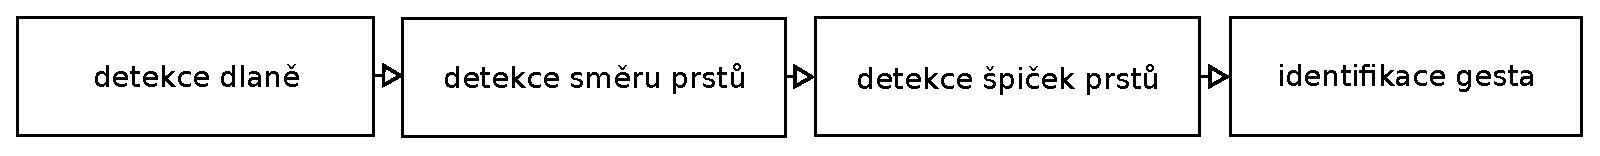
\includegraphics[width=.99\textwidth]{postup.eps}
\caption{Postup nalezení ruky a identifikace gesta }
\label{picPostup}
\end{figure}

\subsubsection{Identifikace gesta}
Gesta lze rozlišovat na statická a dynamická. Pro dynamická gesta je třeba udržovat si v paměti minulé stavy a stanovit dobu, po kterou by bylo přijatelné pro uživatele provádět gesto a zároveň  nemohlo být mylně identifikované. Nejjednodušší je identifikovat gesta statická, kde s využitím euklidovských vzdáleností lze vypočítat počet prstů, a tak v základní verzi bude prostor pro minimálně pět variant, pokud se pro zjednodušení vyloučí zavřená pěst. Program s implementovanou identifikací jednotlivých prstů poskytuje více variant, než by bylo potřeba, nebo by bylo zapamatovatelné pro uživatele.

Počet prstů lze spočítat po správné identifikaci jednotlivých prstů, a jedná se o nejjednodušší způsob klasifikace gesta. Pro přesnost se lze opřít i o úhly a vzdálenosti mezi středem dlaně a špičkami prstů podle vzorců uvedených v kapitole 2.1.4 u obrázku~\ref{pic8}.

Sledováním polohy dlaně v následných snímcích lze detekování gesta zefektivnit. Za předpokladu, že se člověk pohybuje pomaleji, než se střídají snímky k analýze, lze procházet menší část pole, například jen okolí místa, kde se posledně nacházela ruka s prsty a kontrolovat změny, zda počet ukázaných prstů se zmenšil nebo zvětšil. K tomuto účelu by stále stačilo gesto definované počtem prstů bez závislosti na tom, o které konkrétně se jedná.

Otázkou je i jak je definováno gesto. Jedná-li se o číslo, které představuje počet vztyčených prstů, je to nejjednodušší. Může to být ale i objekt, který obsahuje pět prstů, z nichž každý může být zvednutý nebo nikoliv. Pak je podstatně přehlednější implementace více než pěti gest. Identifikace je ale náročnější, jelikož každý nalezený prst se musí nejdříve identifikovat, poté aktualizovat objekt představující ruku před kamerou a porovnat s implementovanými gesty. 

\subsubsection{Vykreslení ruky}
Objekty se přes video vykreslují pomocí FBO ("frame buffer object"). Jedná se o buffery s objekty, které je třeba vykreslit. Reprezentují plátno, na které se příkazy \textit{begin}() a \textit{end}() vykreslují 3D objekty a jednou za snímek či méně často (podle požadavků) se vykreslí příkazem \textit{draw}(). Pro lepší přehled se mohou jednotlivé prsty (konečky prstů) zvýraznit koulí, zatímco celá ruka krychlí. Vykreslují se pouze základní objekty, které upřesňují nalezenou pozici rukou a prstů, aby nebylo potřeba udržovat v paměti přesné okraje ruky, které nejsou pro detekci gesta potřeba.

\section{Předzpracování obrazu}

Kvůli přehlednější práci s matematickými parametry obrazu se nejdříve načtou data z kamery, která jsou uložena v jednodimenzionálním poli a transformují se do dvoudimenzionálního pole pro další zpracování. Přepis je potřeba kvůli práci se souřadnicemi.\\

\subsection{Filtrace}
Chybné hodnoty načtené z kamery je potřeba nejdříve co nejvíce eliminovat. Za tímto účelem je použit medián z okolí.\\

Velikost okolí je zvolena empericky. Čím větší okolí, tím více je výsledek rozmazaný, ale zato obsahuje menší počet odchýlených hodnot, které by mohly narušit průběh zpracování. Pokud se vezme okolí malé, zůstane jich více, ale lépe se zachovají tvary. Na následujících obrázcích lze pozorovat rozdíl mezi okolím 9 (obrázek ~\ref{pic10}) a okolím 25(obrázek ~\ref{pic11}).\\

\begin{figure}[htp]
\centering
\fbox{\includegraphics[width=.4\textwidth]{3-neigh9/befOUT.png}} \hfil
\fbox{\includegraphics[width=.4\textwidth]{3-neigh9/afOUT.png}}
\caption{Medián vypočítaný z okolí mohutnosti 9 \\ a) originální obraz b) po úpravě}
\label{pic10}
\end{figure}
\begin{figure}[htp]
\centering
\fbox{\includegraphics[width=.4\textwidth]{4-neigh25/befOUT.png}} \hfil
\fbox{\includegraphics[width=.4\textwidth]{4-neigh25/afOUT.png}}
\caption{Medián vypočítaný z okolí mohutnosti 25 \\ a) originální obraz b) po úpravě}
\label{pic11}
\end{figure}

\subsection{Prahování}
Pro manipulaci s nalezenými tvary a výpočty mezi jednotlivými body je snazší pracovat s binárním obrazem. Nejdříve se obraz projde a najde nejbližší objekt (maximální hodnota). Díky předchozí filtraci nezkreslí tuto hodnotu žádný špatně detekovaný pixel, který by měl větší hodnotu. Následně se již porovná každý jednotlivý pixel s hodnotou a vytvoří se pole s hodnotami 1 a 0.

Jelikož lze předpokládat, že člověk nebude mít vždy ruku striktně kolmo k pohledu kamery, je záhodno odečíst od hodnoty představující vzdálenost ruky toleranci. Výsledná hodnota tedy záleží na tom, zda původní pixel byl blíže, než nejbližší objekt s ohledem na odchylku. Tolerance není závislá na vzdálenosti ruky od kamery.\\
Na obrázcích~\ref{pic12},~\ref{pic13} a~\ref{pic14} lze pozorovat změny s ohledem na různé tolerance naklonění ruky. S tolerancí 10 je vidět, že kus dlaně chybí, při toleranci 15 je s rukou načtený i znatelný kus předloktí a k tomu i nejednotný kus jiného objektu. Při toleranci pouze 12 je stále detekováno mnoho pixelů a tak je zvolena 10 jako nejlepší tolerance.\\

\begin{figure}[htp]
\centering
\fbox{\includegraphics[width=.3\textwidth]{5-depth-10/befOUT.png}} \hfill
\fbox{\includegraphics[width=.3\textwidth]{5-depth-10/afOUT.png}} \hfill
\fbox{\includegraphics[width=.3\textwidth]{5-depth-10/binOUT.png}}
\caption{Prahování s odchylkou 10 \\ a) originální obraz b) po filtraci c) binární obraz}
\label{pic12}
\end{figure}
\begin{figure}[htp]
\centering
\fbox{\includegraphics[width=.3\textwidth]{7-depth-12/befOUT.png}} \hfill
\fbox{\includegraphics[width=.3\textwidth]{7-depth-12/afOUT.png}} \hfill
\fbox{\includegraphics[width=.3\textwidth]{7-depth-12/binOUT.png}}
\caption{Prahování s odchylkou 12 \\ a) originální obraz b) po filtraci c) binární obraz}
\label{pic13}
\end{figure}
\begin{figure}[htp]
\centering
\fbox{\includegraphics[width=.3\textwidth]{6-depth-15/befOUT.png}} \hfill
\fbox{\includegraphics[width=.3\textwidth]{6-depth-15/afOUT.png}} \hfill
\fbox{\includegraphics[width=.3\textwidth]{6-depth-15/binOUT.png}}
\caption{Prahování s odchylkou 15 \\ a) originální obraz b) po filtraci c) binární obraz}
\label{pic14}
\end{figure}
\newpage
\section{Detekce ruky}
Definujeme-li ruku jako nejbližší objekt, pak je nalezena již při prahování. Pro lepší názornost se ukládá umístění objektu pomocí pole souřadnic pixelů. Pole obsahuje nalezené pixelů, které patří objektu. V programu je vizualizován červeným čtvercem, který má velikost odvozenou od velikosti pole a střed v souřadnicích $ X_{avg}, Y_{avg} $, které jsou vypočteny jako průměr ze všech souřadnic pixelů, které patří objektu. 
Na následujících obrázcích je vidět rozdíl mezi vyhledáváním v originálních datech a nebere v potaz chybné hodnoty a vyhledáváním v binárním obraze s vyfiltrovaným šumem.
\begin{figure}[htp]
\centering
\fbox{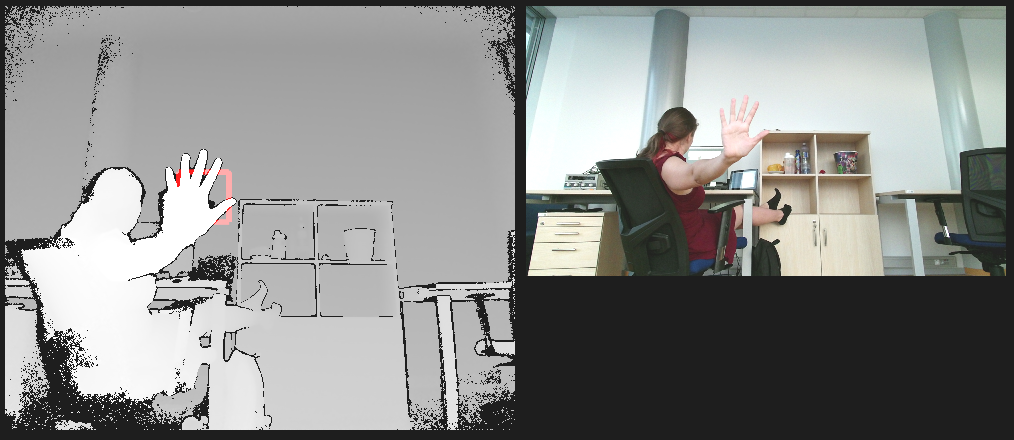
\includegraphics[width=.8\textwidth]{inDepth.png}}
\caption{Obrázek ukazuje největší nalezený nejbližší objekt z originálních dat.}
\label{pic15}
\end{figure}
\begin{figure}[htp]
\centering
\fbox{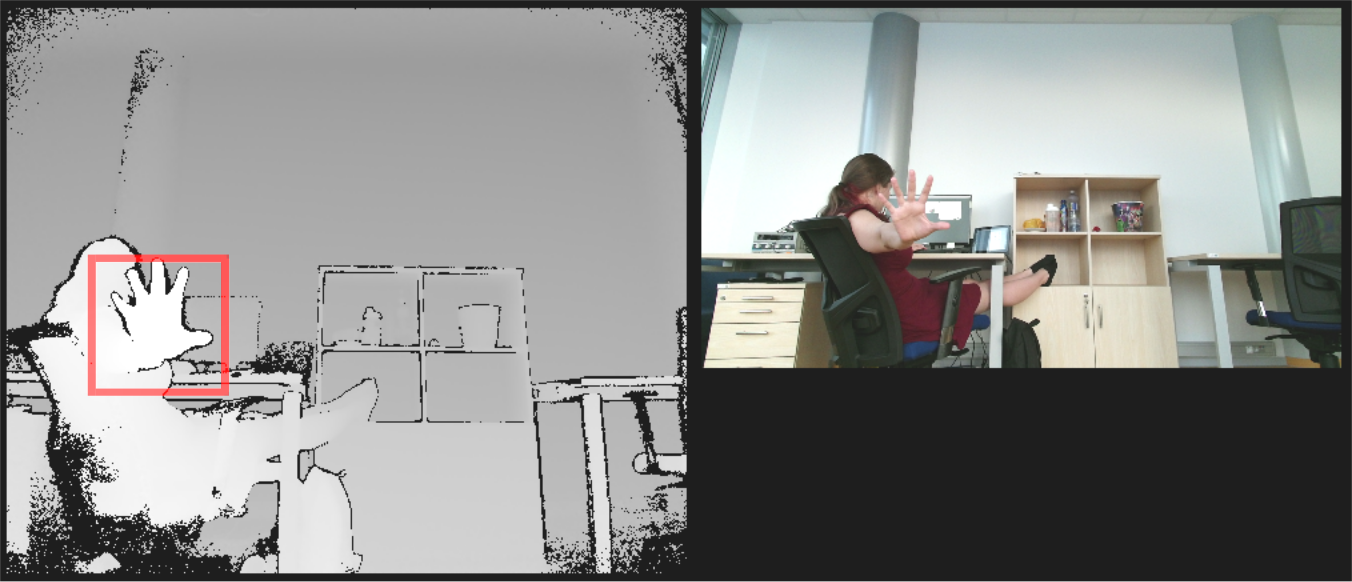
\includegraphics[width=.8\textwidth]{inBinary.png}}
\caption{Největší nejbližší objekt nalezený v binárních vyfiltrovaných datech.}
\label{pic16}
\end{figure}

Z obrázků~\ref{pic15} a~\ref{pic16} lze poznat, že vyhledávání ve filtrovaných datech je přesnější.
\newpage
\section{Detekce dlaně}
V binárním obraze se vyhledá největší plný čtverec, který lze považovat za dlaň. Vytvoří se pomocná matice, do které se zapíší krajové hodnoty binárního obrazu a poté se binární pole prochází z levého horního rohu. Pokud je na dané pozici binárního obrazu nula, přepíše se i do matice. Pokud je tam ale jedna, pak se nalezne minimum třech sousedů z levého horního rohu. To znamená minimum z horního, levého a šikmo horního nalevo. K minumu se přičte jednička, čímž se zvětší velikost čtvercové matice. Ve výsledku tak největší číslo, které je nalezené v pomocné matici, představuje pravý dolní roh největší nalezené matice a zároveň její velikost~\cite{23}. Pro lepší práci v budoucnu je dlaň uložená jako středový bod a velikost matice.

\begin{figure} [htp]
%\begin{subfigure}[b][0.2\textwidth]
\centering
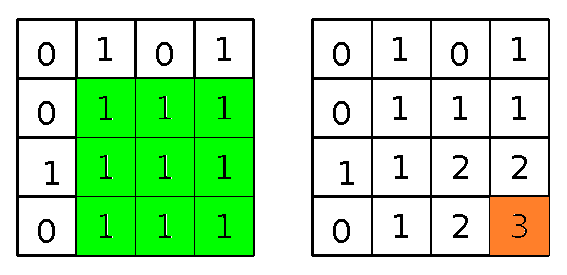
\includegraphics[width=.45\textwidth]{find_palm.eps}
%	\caption{a) původní matice}
%\end{subfigure}
%\begin{subfigure}[b][0.2\textwidth]
%\caption{b) výsledná matice}
%\end{subfigure}
\centering
\caption{Nalezení největší jednotkové matice v binárním obraze. Na levé mapě je binárního obrazu, na kterém se hledá největší plný čtverec (znázorněn zeleně). Vpravo na pomocné matici je detekován pravý dolní konec největšího čtverce (znázorněn oranžově) a jeho velikost je výsledná hodnota (velikost tři pixely). }
\label{pic17}
\end{figure}

Detekce dlaně je vyznačena zeleným čtvercem, jenž má velikost nalezené jednotkové matice a jeho střed má souřadnice $ X_{c}, Y_{c} $, které budou následně využívány jako střed dlaně.

\begin{figure}[htp]
\centering
\fbox{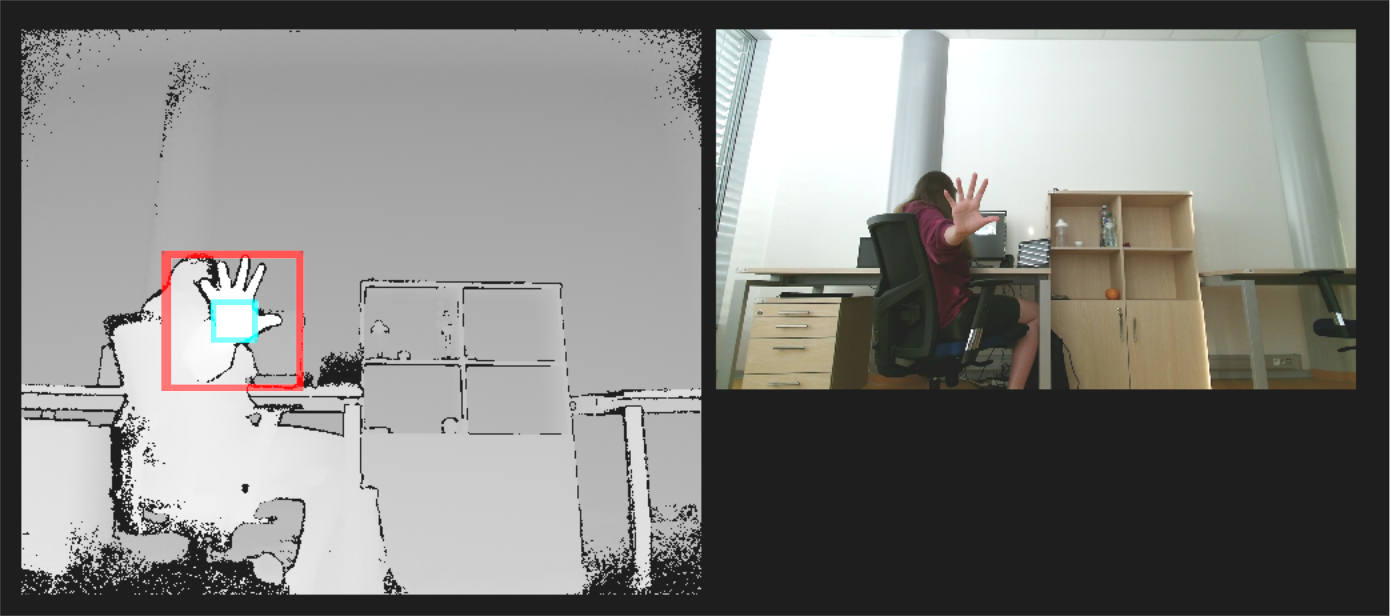
\includegraphics[width=0.8\textwidth]{square.png}}
\caption{Červený čtverec znázorňuje polohu a velikost nalezeného nejbližšího objektu.\\
Zelený čtverec obkresluje největší nalezený čtverec v objektu.}
\label{pic18}
\end{figure}

\section{Oblast zájmu (ROI)}
Po nalezení předpokládaného umístění dlaně se celá oblast označí jako oblast zájmu ('region of interest'). Tato oblast je překopírována do vlastního pole nad kterým pak probíhají další algoritmy. Tímto překopírováním se nepatrně zrychlí běh programu (vetší předvídatelnost přednačítání mezipaměti, méně argumentů ve volání funkcí), ale hlavní výhoda spočívá v jednoduší údržbě navazujících algortimů.

\section{Detekce prstů}
V aplikaci je implentováno několik způsobů nalezení prstů. Pouze některé jsou efektivní a použity ve finální verzi programu, ale pro různost postupu jsou zde uvedeny. Pro všechny byly použity předchozí úpravy obrazu a detekce směru prstů.

\subsection{Detekce směru prstů}
Za předpokladu, že jsou prsty nezaměnitelně užší, než předloktí, lze okolo dlaně ve vzdálenosti $ offset\_palm $ od okraje vést čáru ve všech čtyřech směrech (viz obrázek~\ref{pic19}). Následně se iteruje podél jedné hodnoty souřadnice (pro horizontální směr se jedná o souřadnici \textit{y}) v každém směru a detekují změny v binárním obraze. Pokud jednotlivý nalezený objekt má šířku větší než je třetina šířky dlaně, jedná se o část předloktí a nezapočítává se. Zbylé objekty se zaznamenávají do počtu předpokládanách prstů.  Pro přesnější detekci se daný algoritmus provede ještě jednou pro větší vzdálenost od dlaně. Pokud je pro obě vzdálenosti počet detekovaných prstů větší, než nula, je daný směr zaznamenán. Jelikož je potřeba znát i pozici palce, ukládají se dva směry prstů.

Empiricky nalezená nejlepší hodnota pro $ offset\_palm $ je $ \frac{5}{7} $ šířky dlaně, v druhém kole je zvolena dvojnásobná hodnota. 

\begin{figure}[htp]
\centering
\fbox{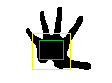
\includegraphics[width=.4\textwidth]{whereFingersAt.png}}
\caption{Zelený čtverec představuje hranice nalezené dlaně. Procházením podél žluté čáry, která je posunuta o offset se počítá počet změn a kontroluje tloušťka nalezených objektů. Pokud tlouťka odpovídá méně než třetině šířky dlaně, pak se považuje za prst.}
\label{pic19}
\end{figure}
\newpage
\subsection{Detekce konců prstů}
Všechny postupy se zakládají na prohledávání v okolí dlaně. Maximální délka prstů se odvozuje od nalezené velikosti dlaně. Prsty nesmí být ani příliš dlouhé ani příliš krátké.\\

%findFingerTips
\subsubsection{Nejvýše položený bod}
Nejjednodušší postup spočívá v rozdělení strany, na které se nachází prsty, na čtyři části, kde každá náleží jednotlivým prstům. Rozdělení je rovnoměrné a nepodporuje tak extrémní odchylky. Celkový obdélník musí být širší než dlaň a nebere se v potaz, který prst je v daném obdélníku nalezen. To znamená, že pokud se ukazují dva prsty, přičemž se některý/oba nachází ve vedlejším obdélníku, zaznamená se správně pouze počet prstů.

Jednotlivé části se následně procházejí a hledá se pixel, který ještě patří prstu a je nejvýše/nejníže dle orientace.\\

\begin{figure}[htp]
\centering
\fbox{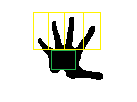
\includegraphics[width=.4\textwidth]{findFingerTips.png}}
\caption{Zelený čtverec představuje nalezenou dlaň. Žluté obdélníky jsou předpokládané pozice prstů na základě nalezeného směru.}
\label{pic20}
\end{figure}

%findFingerTips2
\subsubsection{Nejvzdálenější bod}
Další způsob rozšiřuje využitelnost předchozí metody. Stále se prochází oblast, ve které byly detekovány prsty, ale celkový obdélník se předá v kuse a hledá se největší vzdálenost mezi nalezeným bodem a středem dlaně. Stále platí omezení délky, tudíž je přesnější největší možná vzdálenost, která stále patří prstu.

%findFingerTips3
\subsubsection{Nejvzdálenější bod dle pozice prstu}
Funkce findFingerTips3 si ukládá souřadnice, na kterých byly detekovány prsty z předchozí kapitoly (detekce směru prstů). Následně si dopočítá střed prstu a po přímce prohledává binární obraz tak daleko, dokud nenarazí na konec prstu (nulu v binárním obraze). 

%findFingerTips4
\subsubsection{Nejvzdálenější bod z povoleného okolí}
Další implementovaná možnost nalezení konců prstů spočívá v procházení oblasti, ve které se nachází prsty. Oblast je vyznačena žlutě na obrázku~\ref{pic20}. Hledání začíná u vnější strany dané oblasti a jakmile se narazí na pixel patřící objektu, uloží se jeho pozice a souřadnice se zapíše do pomocného pole. Pole obsahuje souřadnice, na kterých se nachází již nalezené prsty a navíc jejich okolí, ve kterých se stále jedná o ten stejný prst. Při následujícím nalezení pixelu patřícího k objektu se tedy nejdříve zkontroluje, jestli se nejdná o kolizi z pohledu již nalezených prstů.

\subsection{Identifikace prstů}
Index prstu se přidělí podle pozice špičky prstů vzhledem ke středu dlaně viz obrázek~\ref{pic20}. Jelikož není známo, jakým směrem je ruka natočena ke kameře, není identifikovatelné, jestli se jedná o malíček nebo ukazováček. Indexy tedy představují pouze pozici prstu.

\section{Vyhodnocení výsledků detekce gest}
Vyhodnocení funkčnosti a použitelnosti navržených metod.
TODO

\endinput
%%
%% End of file `ch01.tex'.
